\documentclass[conference]{IEEEtran}
\usepackage{graphicx}
\usepackage{amsmath}
\usepackage{hyperref}

\title{Lab 4: 3D Pulmonary Nodule Detection\\Using U-Net on LUNA16 Dataset}
\author{Tran Huy Quan - 22BA13260}

\begin{document}

\maketitle

\section{Introduction}

Lung cancer is one of the leading causes of death worldwide. Detecting lung nodules early from CT scans can significantly improve patient survival rates. However, manually reviewing hundreds of CT slices is time-consuming and prone to human error.

In this lab, we build an automated system that can detect lung nodules from 3D CT scan images. We use a deep learning model called U-Net, which learns to identify suspicious regions in the scans. The model takes in small 3D patches from CT images and outputs a mask highlighting where the nodules are located.

\section{Dataset}

We use the LUNA16 dataset, which is a publicly available collection of lung CT scans with expert-labeled nodule locations. Specifically, we work with \textbf{subset0}, which contains 89 CT scans stored in \texttt{.mhd} format.

The annotations file provides the world coordinates (X, Y, Z) and diameter (in mm) of each nodule. We filter the annotations to only include nodules from subset0.

\subsection{Data Preparation}

The raw CT images are in Hounsfield Unit (HU) scale. We normalize the pixel values to a 0--1 range by clipping the values between --1000 and 400 HU.

For each nodule, we extract a small 3D cube (patch) of size $32 \times 32 \times 32$ voxels centered at the nodule location. We also create a corresponding ground truth mask --- a sphere centered at the nodule position, with a radius based on the annotated diameter.

To help the model learn what ``no nodule'' looks like, we also extract negative patches from random locations in the same CT scan, with empty masks (all zeros). This gives us a balanced dataset with both positive and negative examples.

\section{Model Architecture}

We use MONAI's \textbf{BasicUNet}, a 3D version of the popular U-Net architecture. The model works like an encoder-decoder:

\begin{itemize}
    \item \textbf{Encoder}: Gradually compresses the input image to capture important features at different scales.
    \item \textbf{Decoder}: Expands the compressed features back to the original size, producing a pixel-level prediction map.
    \item \textbf{Skip connections}: Connect matching layers between encoder and decoder to preserve fine details.
\end{itemize}

The model has the following configuration:
\begin{itemize}
    \item Input: 1-channel 3D patch ($1 \times 32 \times 32 \times 32$)
    \item Output: 1-channel prediction mask (same size as input)
    \item Feature sizes: (16, 16, 32, 64, 128, 16)
\end{itemize}

\section{Training}

\subsection{Training Setup}

\begin{itemize}
    \item \textbf{Train/Validation split}: 80\% training, 20\% validation
    \item \textbf{Batch size}: 2
    \item \textbf{Learning rate}: 0.001
    \item \textbf{Epochs}: 3
    \item \textbf{Loss function}: Dice Loss + 0.5 $\times$ Binary Cross-Entropy Loss
    \item \textbf{Optimizer}: Adam
\end{itemize}

The combined loss function helps the model learn both the overall shape (Dice Loss) and the individual pixel predictions (BCE Loss) of the nodules.

\subsection{Training Results}

Figure~\ref{fig:training} shows the training curves over 3 epochs. The training loss decreases steadily from approximately 1.18 to 1.02, indicating that the model is learning. The validation Dice score starts low (around 0.05) and improves to approximately 0.30 by the end of training, showing that the model gradually gets better at matching its predictions with the ground truth masks.

\begin{figure}[h]
    \centering
    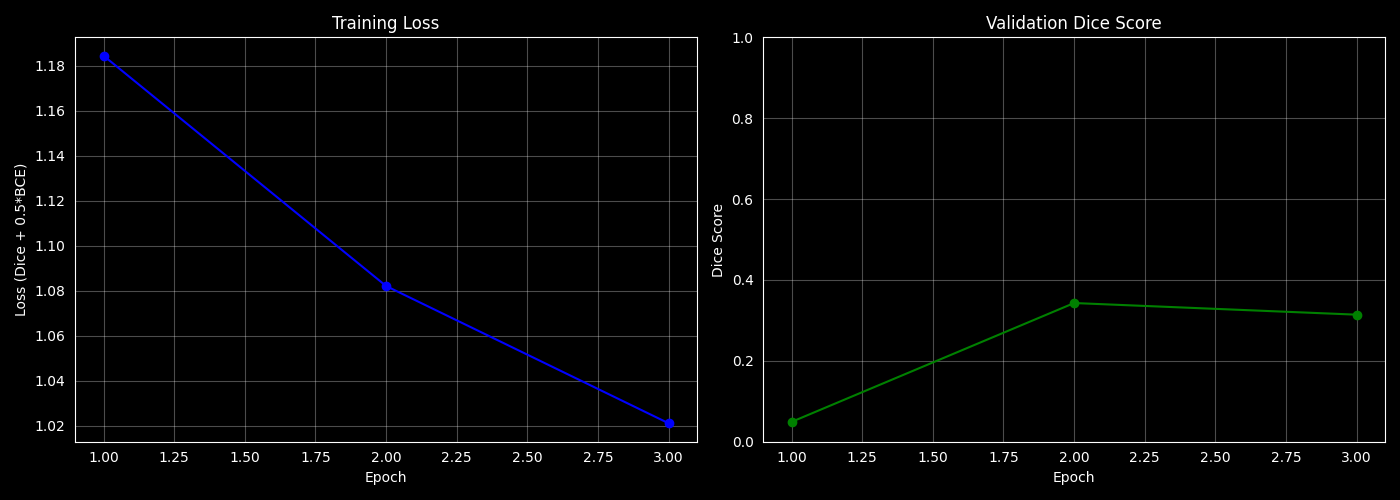
\includegraphics[width=\columnwidth]{training_curves.png}
    \caption{Training loss (left) and validation Dice score (right) over 3 epochs.}
    \label{fig:training}
\end{figure}

\section{Evaluation and Inference}

After training, we evaluate the model on CT scans from the dataset. The evaluation involves:

\begin{enumerate}
    \item Loading a full CT scan and normalizing it.
    \item Running the model using a sliding window approach --- the model processes the large volume in small overlapping patches of $32 \times 32 \times 32$.
    \item Combining all patch predictions into a full-volume prediction mask.
    \item Post-processing: removing small detected regions (fewer than 10 voxels) that are likely noise.
\end{enumerate}

We measure two metrics:
\begin{itemize}
    \item \textbf{Dice Score}: Measures how well the predicted mask overlaps with the ground truth. Ranges from 0 (no overlap) to 1 (perfect match).
    \item \textbf{Sensitivity}: The percentage of actual nodules that the model successfully detects.
\end{itemize}

\subsection{Inference Visualization}

Figure~\ref{fig:inference} shows an example inference result on a CT scan. The left panel shows the original CT slice, the middle panel shows the model's prediction mask, and the right panel shows the overlay of the prediction on the CT scan, highlighting the detected regions.

\begin{figure}[h]
    \centering
    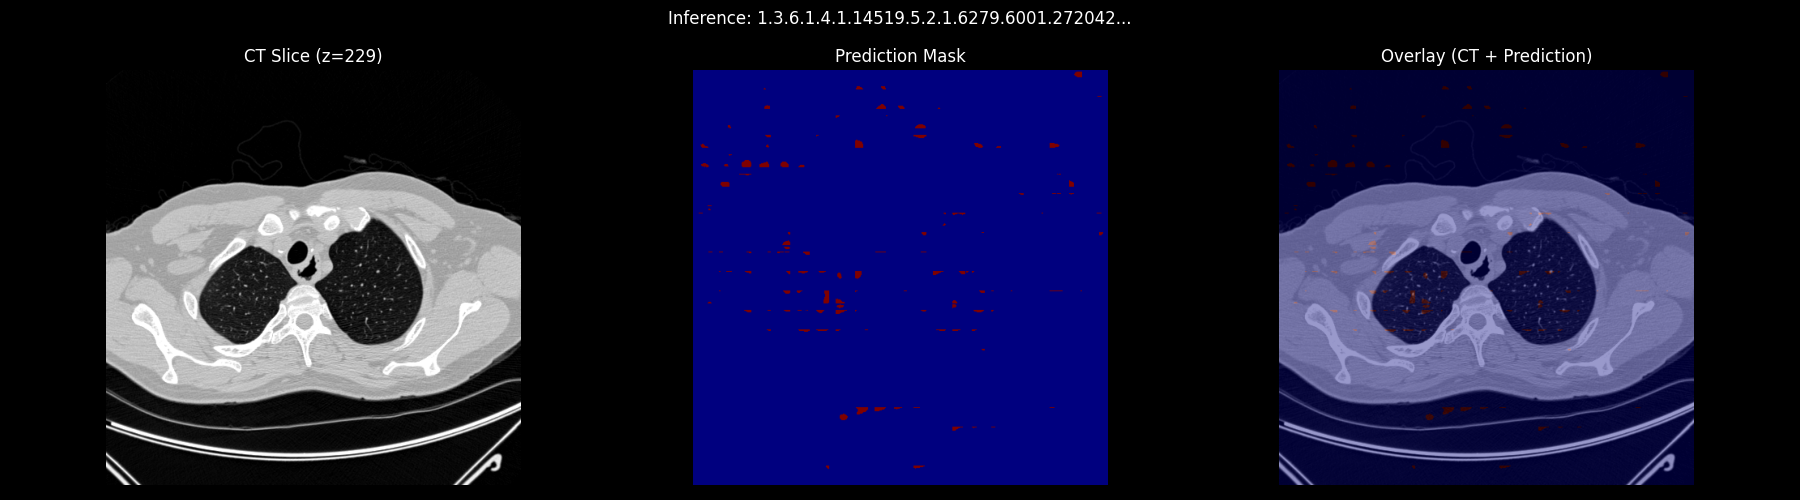
\includegraphics[width=\columnwidth]{inference_1.3.6.1.4.1.14519.5..png}
    \caption{Inference result: CT slice (left), prediction mask (middle), and overlay (right).}
    \label{fig:inference}
\end{figure}

\section{Discussion}

The model shows promising learning behavior with the loss decreasing consistently. However, the Dice score of approximately 0.30 suggests there is room for improvement. Several factors contribute to this:

\begin{itemize}
    \item \textbf{Limited training}: Only 3 epochs were used due to computational constraints. More epochs would likely improve performance.
    \item \textbf{Small patch size}: Using $32 \times 32 \times 32$ patches limits the context the model can see around each nodule.
    \item \textbf{Small model}: The reduced feature sizes mean the model has fewer parameters to learn complex patterns.
    \item \textbf{Dataset size}: Only subset0 (89 CT scans) was used. Using more subsets would provide more training data.
\end{itemize}

Despite these limitations, the model demonstrates that it can learn to identify nodule-like regions from CT data, which validates the overall approach.

\section{Conclusion}

In this lab, we implemented a 3D lung nodule detection pipeline using the U-Net model on the LUNA16 dataset. The pipeline includes data loading, preprocessing, patch extraction, model training, and inference with visualization. While the current results are modest due to computational constraints, the decreasing loss and improving Dice score confirm that the model is learning meaningful patterns. With more training time and data, this approach has the potential to achieve better performance for automatic nodule detection.

\end{document}
